\documentclass{article}

%\documentclass{report}
\usepackage{braket}
\usepackage{amsmath}
\usepackage{mathtools}
\usepackage{amssymb}
\usepackage{trsym}
\usepackage{pifont}
\usepackage{tcolorbox}
\usepackage[T1]{fontenc}
\usepackage[utf8]{inputenc}
\usepackage[english]{babel}
\usepackage{amsfonts}
\usepackage[super]{nth}
\usepackage{float}
\usepackage{caption}
\usepackage{graphicx}
\usepackage{subcaption}
\usepackage{geometry}
\usepackage{csquotes}
\usepackage{tikz}
\usepackage{circuitikz}
\usepackage{listings}
\usepackage{bbm}
\usepackage{siunitx}
\usepackage{hyperref}
\makeatletter
\renewcommand\paragraph{\@startsection{paragraph}{4}{\z@}%
	{-2.5ex\@plus -1ex \@minus -.25ex}%
	{1.25ex \@plus .25ex}%
	{\normalfont\normalsize\bfseries}}
\makeatother
\setcounter{secnumdepth}{4} % how many sectioning levels to assign numbers to
\setcounter{tocdepth}{4}    % how many sectioning levels to show in ToC
\usetikzlibrary{decorations.pathmorphing}
\geometry{
	a4paper,
	total={150mm,237mm},
	left=30mm,
	top=25mm,
}

\graphicspath{{imgs/}}

\DeclareMathOperator{\var}{Var}

\title{Harmonic Oscillator}
\author{Benedikt Otto}


\begin{document}
	\maketitle
	\newpage
	\tableofcontents
	\newpage
	\begin{abstract}
		To evaluate the behaviour of a quantum particle in a certain potential the path-integral method can be used.
		In this project I investigated the behaviour of particles in a harmonic and anharmonic potential.
		I measured the ground state energy and the corresponding autocorrelation.
		Additionally I examined the tunnelling behaviour of the anharmonic oscillator for different distances of the minima.
		To verify my code I used the classical limit corresponding to $\hbar \rightarrow 0$.
	\end{abstract}
	\section{Introduction}
	\section{Theoretical Basis}
		It corresponds to the generalisation of the principle of the least action in classical mechanics.
		%However the solution in quantum mechanics does not yield a defined path, rather 
		\begin{equation}
			K(a, b) = \int_a^b e^{iS/\hbar} \mathcal Dx(t)
			\label{eq:path_integral}
		\end{equation}
		In equation \ref{eq:path_integral} the integral is performed over the path from point $a$ to $b$.
		\\
		The total action is given by equation \ref{eq:total_action}.
		\begin{equation}
			S = \epsilon \sum_{i=0}^{N - 1} \left(\frac{m(x_{i+1} - x_i)^2}{2\tau^2} + V(x_i)\right)
			\label{eq:total_action}
		\end{equation}
		Because the analysis is more convenient, often periodic boundary conditions are used.
		In this case one can define $x_0 = x_N$, so the right neighbour of $x_{N-1}$ is $x_0$.
		The left part of the equation corresponds to the kinetic energy.
		The velocity used is the average velocity, when the particle moves from site $x_i$ to $x_{i+1}$.
		Because every change only affects three terms, it is not necessary to recalculate the complete action for every change.
		\begin{equation}
			\begin{split}
				\Delta S(x_{i-1}, x_i, x'_i, x_{i+1}) =\\
				\tau\left(V(x_i) - V(x'_i) + m\frac{(x_{i-1} - x_i)^2 + (x_i - x_{i+1})^2 - (x_{i-1} - x'_i)^2 - (x'_i - x_{i+1})^2}{2\tau^2}\right)
			\end{split}
			\label{eq:delta_total_action}
		\end{equation}
		This rewrite reduces the complexity of the problem and improves performance.
		The time complexity per Metropolis iteration is thus reduced from $\mathcal O(n^2)$ to $\mathcal O(n)$, where n corresponds to the number of lattice cites.
	\section{Methods}
		To generate the track data the \textbf{Metropolis} algorithm is used:

		At first the positions of the particle at every time step is initialised to a random distribution.
		Then for every time step a new position is drawn from a random distribution, in this case from a gaussian distribution.
		If this change lowers the total \textbf{action}, calculated over all the time lattice points, the change is accepted.
		Otherwise, a linearly distributed random value is drawn in the range from 0 to 1 and compared to the exponent of the difference in the \textbf{action}, divided by $\hbar$.
		If the random variable is smaller than the exponential function, the value is accepted, otherwise is is rejected and the position at that time step not updated.
		This behaviour leads to the tendency to thermalise, but takes care of the quantum behaviour of the particle.
	\section{Implementation}
		At first I implemented the complete algorithm in \textbf{Python}, which leads to a fairly poor performance.
		This could mean that one can only get a bad data quality in a given time.
		Thus I optimised the code for performance by simplifying the energy term and precalculating the random variables.
		This reduced the execution time of around 35\%.
		Since this is still a poor performance, I implemented the main Metropolis algorithm loop in \textbf{C++}, the higher level computation is still done in \textbf{Python}.
		For the interfacing the library \verb!ctypes! is used.
		This change improved the total performance, including the still in Python performed generation of the plots, by a factor of around 8.
		This leads to an improvement of data quality due to the higher output rate of around one order of magnitude.
		The complete source code, including all files related to this project are available under the public github repository \cite{github}.
		To verify that the \textbf{C++} code behaves exactly like the Python version, I created some tests, stored in the branch \verb!verify_C!.
	\section{Results}
	\begin{figure}[htbp]
		\centering
		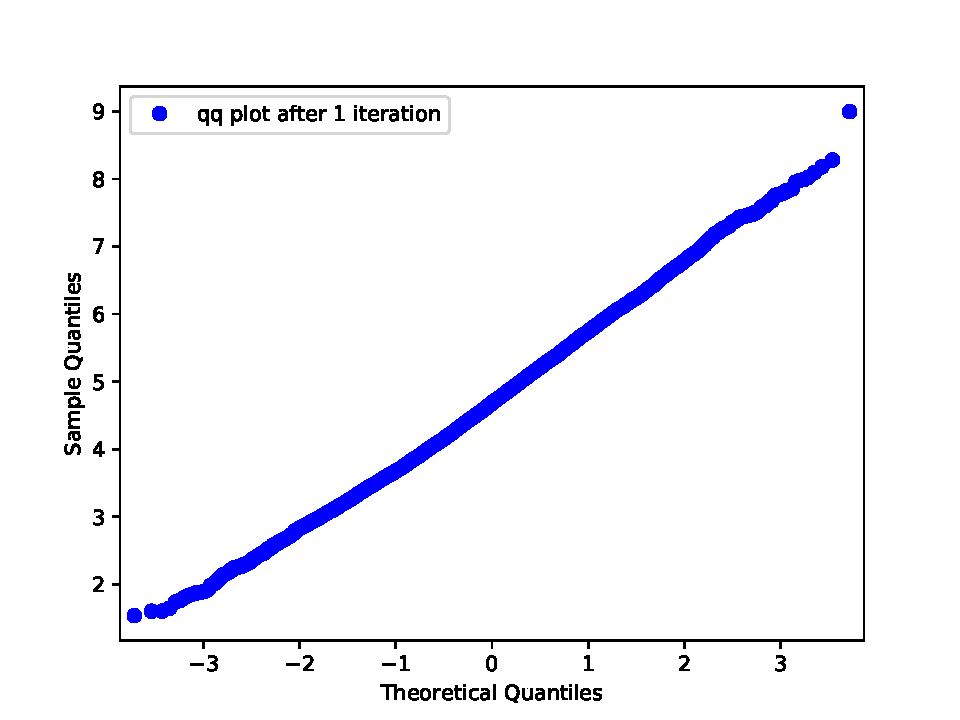
\includegraphics[width=0.4\textwidth]{../imgs/harmonic_oscillator_track/track_10010000_qq_1.pdf}
		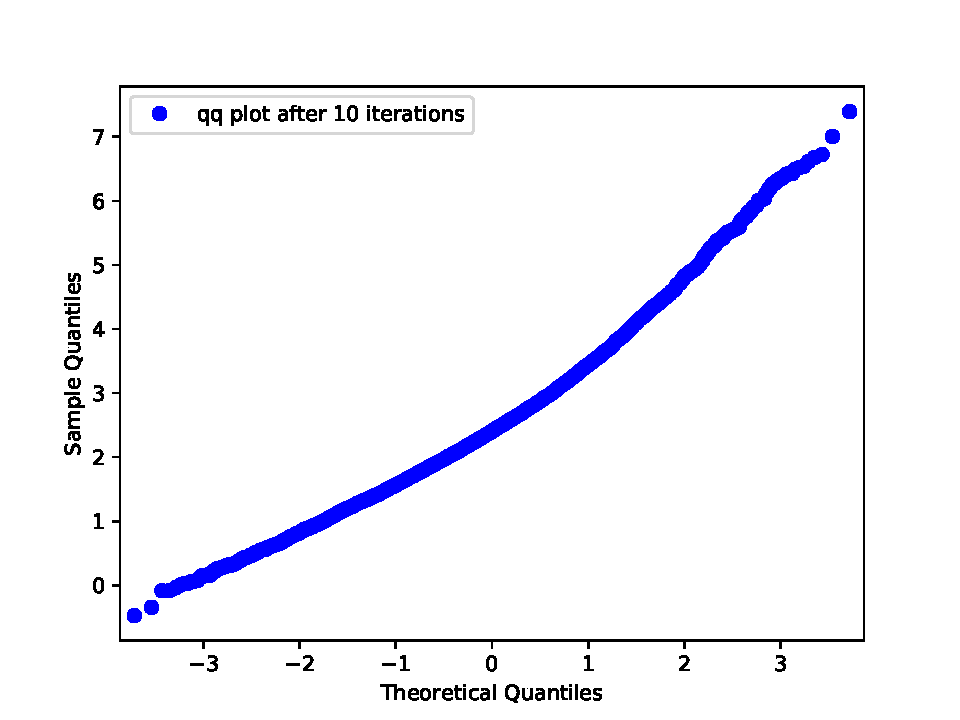
\includegraphics[width=0.4\textwidth]{../imgs/harmonic_oscillator_track/track_10010000_qq_10.pdf}
		\\
		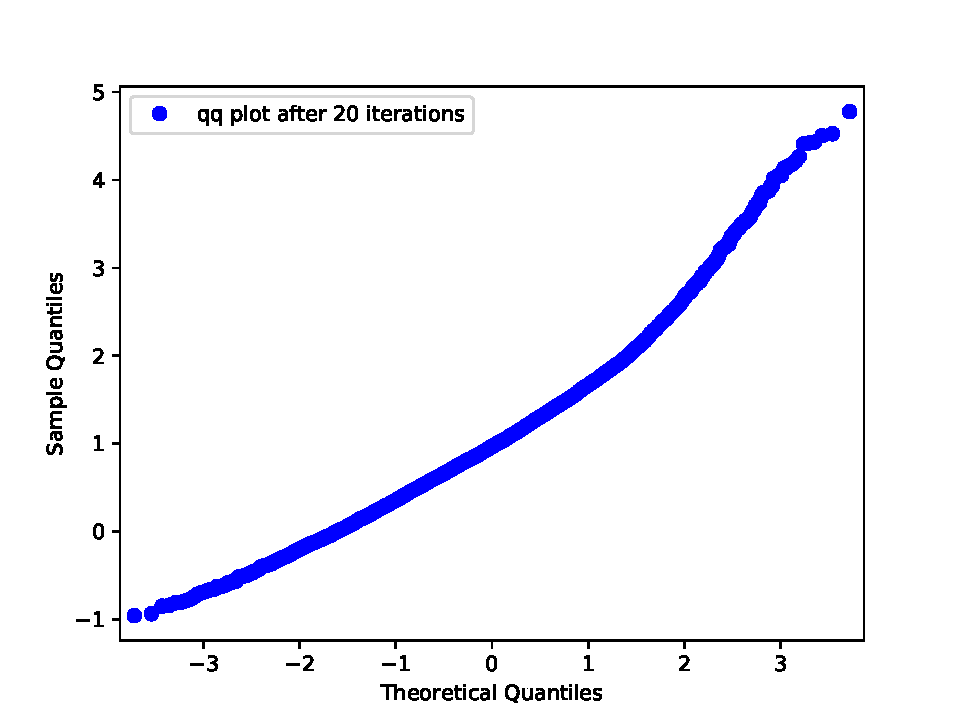
\includegraphics[width=0.4\textwidth]{../imgs/harmonic_oscillator_track/track_10010000_qq_20.pdf}
		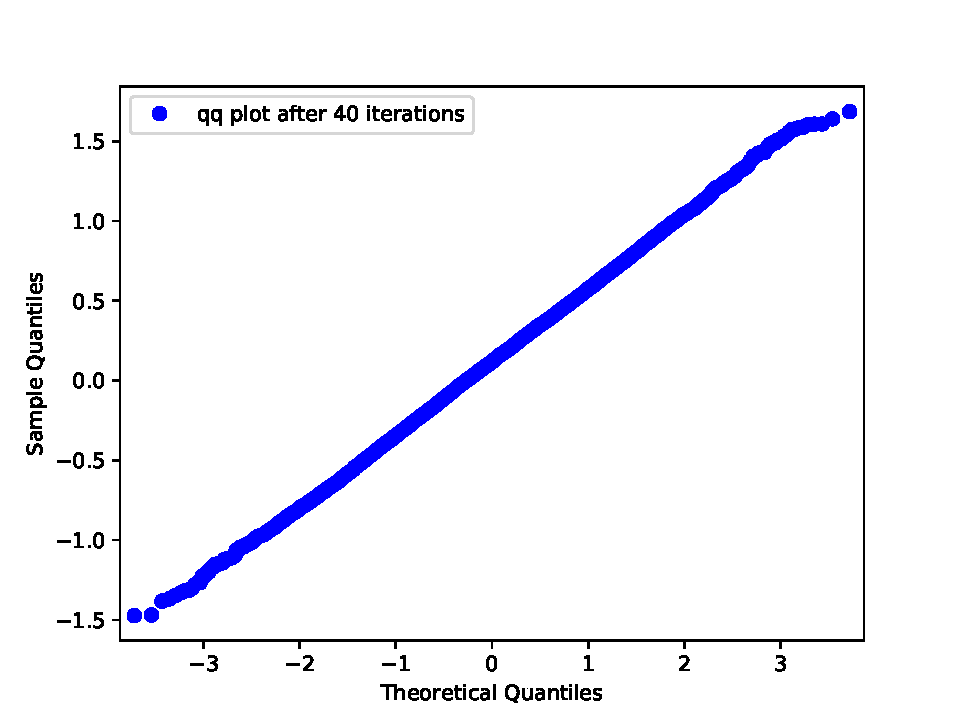
\includegraphics[width=0.4\textwidth]{../imgs/harmonic_oscillator_track/track_10010000_qq_40.pdf}
		\\
		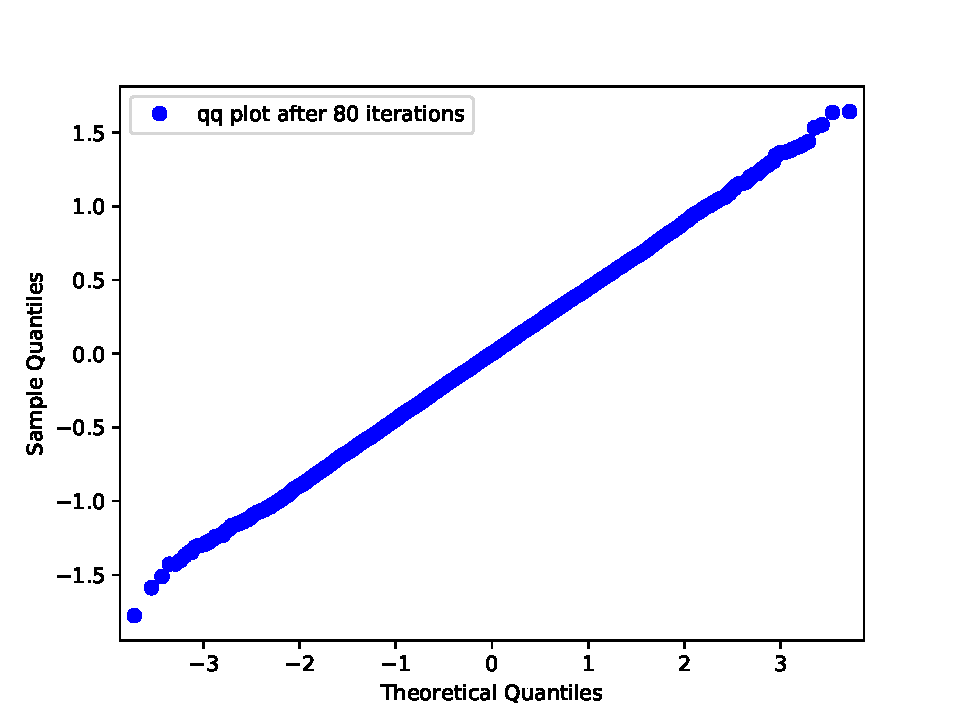
\includegraphics[width=0.4\textwidth]{../imgs/harmonic_oscillator_track/track_10010000_qq_80.pdf}
		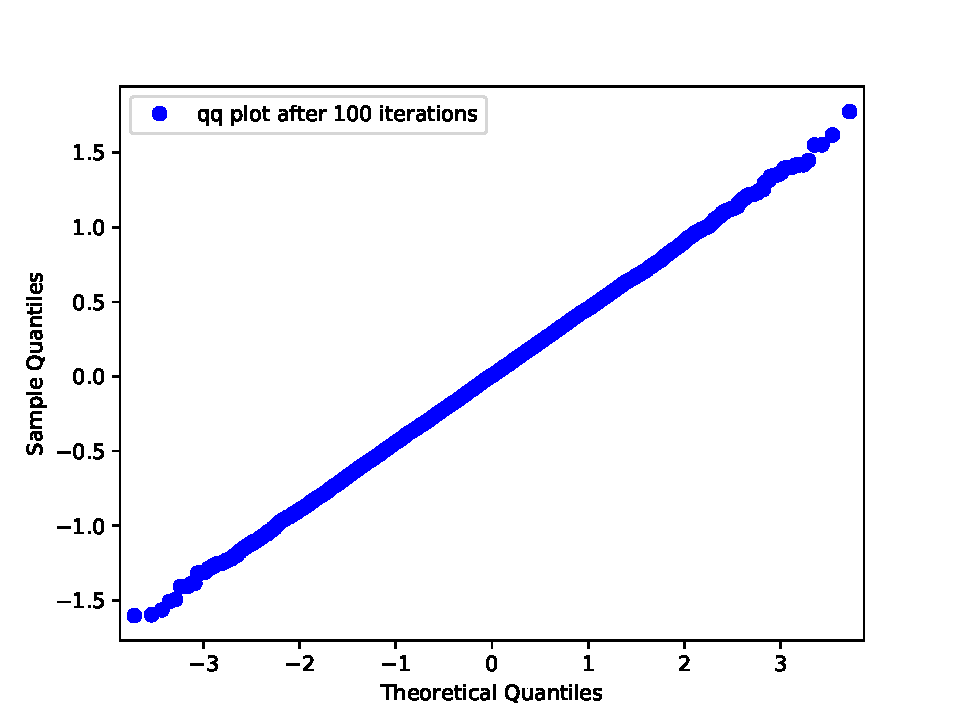
\includegraphics[width=0.4\textwidth]{../imgs/harmonic_oscillator_track/track_10010000_qq_100.pdf}
		\caption{}
	\end{figure}
	\section{Discussion}
	\section{Summary and Outlook}
	\begin{thebibliography}{widestlabel}
		\bibitem{github} Public Github repository: Harmonic Oscillator, Benedikt Otto (s6beotto), \\\url{https://github.com/s6beotto/Harmonic-Oscillator}.
		\bibitem{latexrun} Public Github repository: latexrun, Austin Clements (aclements), \\\url{https://github.com/aclements/latexrun}.
		\bibitem{creutz_freedman} M. Creutz and B. Freedman, \textit{A statistical approach to quantum mechanics}, Annals of Physics, \textbf{132}, 427-462 (1981).
		\bibitem{rodgers_raes} R. Rodgers and L. Raes, \textit{Monte Carlo simulations of harmonic and anharmonic oscillators in discrete Euclidean time}, DESY Summer Student Programme (2014).
	\end{thebibliography}
	\appendix
	\section{Directory structure}
	\subsection{Data generation}
	\begin{figure}[H]
		\centering
		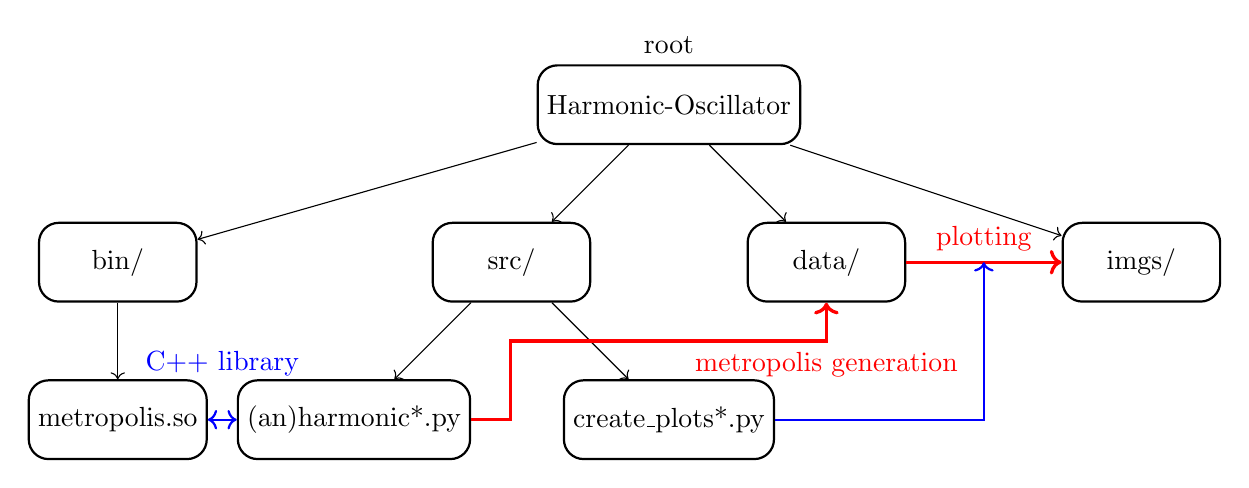
\begin{tikzpicture}
		\draw[color=black, thick]
		node[draw,minimum width=2cm,minimum height=1cm,label=root,rounded corners=0.25cm] (root) at (0, 0){Harmonic-Oscillator}
		node[draw,minimum width=2cm,minimum height=1cm,rounded corners=0.25cm] (bin) at (-7, -2){bin/}
		node[draw,minimum width=2cm,minimum height=1cm,rounded corners=0.25cm] (bin_metropolis) at (-7, -4){metropolis.so}
		node[draw,minimum width=2cm,minimum height=1cm,rounded corners=0.25cm] (src) at (-2, -2){src/}
		node[draw,minimum width=2cm,minimum height=1cm,rounded corners=0.25cm] (src_create) at (-4, -4){(an)harmonic*.py}
		node[draw,minimum width=2cm,minimum height=1cm,rounded corners=0.25cm] (src_plot) at (0, -4){create\_plots*.py}
		node[draw,minimum width=2cm,minimum height=1cm,rounded corners=0.25cm] (data) at (2, -2){data/}
		node[draw,minimum width=2cm,minimum height=1cm,rounded corners=0.25cm] (imgs) at (6, -2){imgs/};
		\draw [->] (root) -- (bin);
			\draw [->] (bin) -- (bin_metropolis);
		\draw [->] (root) -- (src);
			\draw [->] (src) -- (src_create);
			\draw [->] (src) -- (src_plot);
		\draw [->] (root) -- (data);
		\draw [->] (root) -- (imgs);
		\draw [<->, thick, blue] (bin_metropolis) -- (src_create) node[midway,above=12] {C++ library};
		\draw [->, very thick, red] (src_create.east) -| ++(0.5, 1) -| (data) node[midway,below] {metropolis generation};
		\draw [->, very thick, red] (data) -- (imgs) node[midway,above] {plotting};
		\draw [->, thick, blue] (src_plot.east) -| (4, -2);
		\end{tikzpicture}
		\caption{Directory structure of the project for data generation}
		\label{fig:scheme_dirs_data_generation}
	\end{figure}
	\subsection{Report generation}
	\begin{figure}[H]
		\centering
		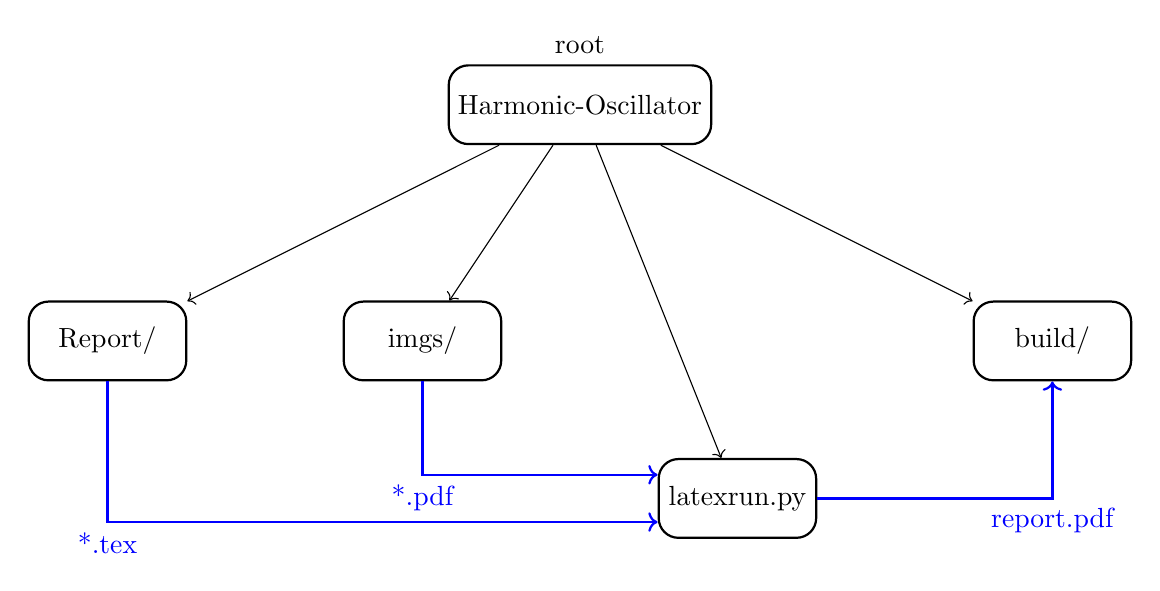
\begin{tikzpicture}
		\draw[color=black, thick]
		node[draw,minimum width=2cm,minimum height=1cm,label=root,rounded corners=0.25cm] (root) at (0, 0){Harmonic-Oscillator}
		node[draw,minimum width=2cm,minimum height=1cm,rounded corners=0.25cm] (report) at   (-6,  -3){Report/}
		node[draw,minimum width=2cm,minimum height=1cm,rounded corners=0.25cm] (imgs) at     (-2, -3){imgs/}
		node[draw,minimum width=2cm,minimum height=1cm,rounded corners=0.25cm] (latexrun) at (2,  -5){latexrun.py}
		node[draw,minimum width=2cm,minimum height=1cm,rounded corners=0.25cm] (build) at    (6,  -3){build/};
		\draw [->] (root) -- (report);
		\draw [->] (root) -- (imgs);
		\draw [->] (root) -- (latexrun);
		\draw [->] (root) -- (build);
		\draw [<-, thick, blue] (latexrun.west) + (0,-3mm) -| (report.south) node[midway,below] {*.tex};
		\draw [<-, thick, blue] (latexrun.west) + (0, 3mm) -| (imgs.south)   node[midway,below] {*.pdf};
		\draw [->, thick, blue] (latexrun) -| (build.south)                  node[midway,below] {report.pdf};
		\end{tikzpicture}
		\caption{Directory structure of the project for report generation}
		\label{fig:scheme_dirs_report_generation}
	\end{figure}
	The file \verb!latexrun.py! is taken from \cite{latexrun}.
\end{document}